\documentclass[12pt]{report}
\usepackage[a4paper]{geometry}
\usepackage{fancyhdr}
\usepackage{graphicx, wrapfig, subcaption, setspace, booktabs}
\usepackage[T1]{fontenc}
\usepackage[font=small, labelfont=bf]{caption}
\usepackage[protrusion=true, expansion=true]{microtype}
\usepackage[english]{babel}
\usepackage{url}

% no chapiters
\usepackage{titlesec}
\titleformat{\chapter}{\normalfont\LARGE\bfseries}{\thechapter}{1em}{}
\titlespacing*{\chapter}{0pt}{3.5ex plus 1ex minus .2ex}{2.3ex plus .2ex}
\usepackage{biblatex}
%\bibliographystyle{plain}
\bibliography{Rapport2Stage_biblio} 

\newcommand{\HRule}[1]{\rule{\linewidth}{#1}}
\onehalfspacing
\setcounter{tocdepth}{5}
\setcounter{secnumdepth}{5}

% diagrams
\usepackage{tikz}
\usetikzlibrary{shapes,arrows,shadows}
\usepackage{amsmath,bm,times}
\newcommand{\mx}[1]{\mathbf{\bm{#1}}} % Matrix command
\newcommand{\vc}[1]{\mathbf{\bm{#1}}} % Vector command

% page numerotation



%-------------------------------------------------------------------------------
% HEADER & FOOTER
%-------------------------------------------------------------------------------
%\pagestyle{fancy}
%\fancyhf{}
%\setlength\headheight{15pt}
%\fancyhead[L]{\textsc{Master's Thesis}}
%\fancyhead[R]{\textsc{Alexandrina Bodrug}}
%\fancyfoot[R]{\textsc{page} \thepage\ } %of \pageref{LastPage}}

\begin{document}

%-------------------------------------------------------------------------------
% TITLE PAGE
%-------------------------------------------------------------------------------
\begin{titlepage}

\title{ 
\includegraphics[width=\textwidth, height=\textheight, keepaspectratio]{logos.jpg} \vspace*{1\baselineskip} \\
        \large \textbf{\textsc{Master's Thesis}} \\
        \normalsize \textsc{University of Rennes 1} \\
        \normalsize \textsc{Bioinformatics and genomics Master's Degree} \\
        \normalsize \textsc{(2014 - 2015)}
		\\
		\HRule{0.5pt} \\
		\large \textbf{\textsc{Visual representation and comparative evaluation of scaffolding tools for circular genomes}}
		\HRule{2pt} \\ [0.5cm]
		\footnotesize \textsc{Institute for Research in IT and Random Systems, Genscale \\
		263 Avenue General Leclerc, 35000 Rennes, France}
        }
\author{ \normalsize
	\begin{minipage}{0.4\textwidth}
	\begin{flushleft} 
	\emph{Author:}\\
	Alexandrina \textsc{Bodrug}
	\end{flushleft}
	\end{minipage}
	~
	\begin{minipage}{0.4\textwidth}
	\begin{flushright}
	\emph{Supervisors:} \\
	\textit{Pr.} R. \textsc{Andonov} \\
	\textit{Pr.} D. \textsc{Lavenier}
	\end{flushright}
	\end{minipage}\\[2cm]
	}
\end{titlepage}
\maketitle
\newpage
%-------------------------------------------------------------------------------
% THX
%-------------------------------------------------------------------------------
Thanks
\thispagestyle{empty}
\newpage
%-------------------------------------------------------------------------------
% ABBRV	 & GITHUB
%-------------------------------------------------------------------------------
Abbreviations \& github link
\thispagestyle{empty}
\newpage
%-------------------------------------------------------------------------------
% ToC
%-------------------------------------------------------------------------------
\tableofcontents
\thispagestyle{empty}
%-------------------------------------------------------------------------------
% BODEH!
%-------------------------------------------------------------------------------
\chapter{Introduction}
\setcounter{page}{1}
\section{Context}
Whole genome shotgun assembly is the process which transforms the small fragmented DNA sequences called reads produced by Next Generation Sequencing methods into relatively unfragmented genomes and chromosomes. The uninterrupted genome sequence is a precious information in many research fields, which explains the plethora of NGS techniques and assembly tools. The assembly process is described in figure~\ref{fig:AssemblySteps}.
\begin{figure}[ht]
\caption{\textsc{Steps of the whole genome shotgut assembly}} \label{fig:AssemblySteps}
\tikzstyle{file}=[draw, fill=orange!10, text width=9em, 
    text centered, minimum height=2em,drop shadow]
\tikzstyle{file2}=[fill=pink!15, text width=25em, minimum height=2.5em]
 \begin{tikzpicture}
\matrix [column sep=50mm, row sep=10mm] {
  \node (rawdata) [file] {\textbf{raw data} \\ \scriptsize generated by the sequencer}; \\
  \node (cleanreads) at (0,4) [file] [fill=orange!20] {\textbf{clean reads} \\ \scriptsize paired end, mate paired \ldots}; \\
  \node (contigs) [file] [fill=orange!30] {\textbf{contigs}}; \\
  \node (scaffolds) [file] [fill=orange!40] {\textbf{scaffolds}}; \\
};
\draw[->, thick] (rawdata) -- (cleanreads);
\draw[->, thick] (cleanreads) -- (contigs);
\draw[->, thick] (contigs) -- (scaffolds);

    \path (rawdata.west)+(9,-1) node (filtering) [file2] {\footnotesize \textbf{Filtering:} reads containing errors, with unsatisfying coverages, maping with the wrong insert size \textit{etc} can be eliminated during this step.};
    \path (cleanreads.west)+(9,-1) node (contigage) [file2] {\footnotesize \textbf{Building contigs:} a contig is a set of overlapping reads forming a contiguous sequence of DNA. Reads can be single or paired with different insert sizes (distance between two reads). Below is an illustration of read pairs (same color arrows) aligned on a DNA sequence in \textit{Forward - Reverse} (1) and  \textit{Reverse - Forward} (2) order.};
\node[inner sep=0pt] (whitehead) at (7,-1.25) {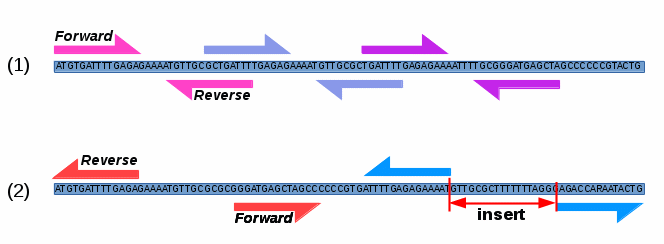
\includegraphics[width=0.60\textwidth]{READS2.png}};
    \path (contigs.west)+(9,-1) node (scaffolding) [file2] {\footnotesize \textbf{Scaffolding:} relative orientation and ordering of contigs.};    
\end{tikzpicture}
\end{figure}\\
Building contigs and scaffolding are two very different problems that were often combined into a single black box tool, in the early years of genome assembly. Many assemblers are in fact just contig builders; the scaffolding methodology being hardly described or accessible. Since the first stand alone scaffolding tools, the importance of scaffolding was underlined. In 2014 researchers from The Wellcome Trust Sanger Institute (Cambridge) conducted a comprehensive evaluation of scaffolding tools then available. New tools are constantly being published. The aim is clear and appears as rather simple: to order and orient contigs. Most tools model the problem as a graph where vertices represent contigs and links represent bundles of pairs of reads linking two contigs. Erroneous data (fake links due to poorly assembled contigs, low quality libraries), missing data (low quality libraries, unfit insert size, low genome coverage) and inherent genome characteristics (repeated regions,  heterozygosity) stand in the way of a perfect and easy scaffolding process. Thus, for an easier scaffolding process, the quality of contigs and the choice of paired end libraries are critical. However the difficulties arising from the sequence structure are to be dealt within the scaffolder.

\section{Aims of the internship project}


\newpage
\section{Workflow}
% Define the layers to draw the diagram
\pgfdeclarelayer{background}
\pgfdeclarelayer{foreground}
\pgfsetlayers{background,main,foreground}
% Define block styles used later

\tikzstyle{file}=[draw, fill=blue!10, text width=7em, 
    text centered, minimum height=2.5em,drop shadow]
\tikzstyle{scaf} = [file, text width=10em, fill=green!20, 
    minimum height=3em, rounded corners, drop shadow]
\tikzstyle{scaf2} = [file, text width=7em, fill=green!20, 
    minimum height=3em, rounded corners, drop shadow]
\tikzstyle{scafli} = [file, text width=10em, fill=cyan!20, 
    minimum height=3em, rounded corners, drop shadow]   

\tikzstyle{ann} = [above, text width=2em, text centered]
\tikzstyle{sc} = [file, text width=13em, fill=red!20, 
    minimum height=10em, rounded corners, drop shadow]

% Define distances for bordering
\def\blockdist{2.5}
\def\edgedist{2.5}

\begin{tikzpicture}

% Genscale 1 step scaffolders
    \node (scaf) [scaf]  {\textsc{\textbf{Scaffolding}}};
    \path (scaf.west)+(-2.5,0) node (gitxt) [file] {\textit{genscaf\_input.txt}}; 
    \path (scaf.east)+(2.5,0) node (ggftxt) [file] {\textit{genome.txt} \\ \scriptsize ordered list of contigs};
    
    \path (gitxt.west)+(-3,-10) node (cfasta) [file] {\textit{contigs\_all.fa} \\ \scriptsize list of contig sequences};  
    
    \path [draw, ->] (cfasta.north)  edge[bend  left=10]  node [left] {\scriptsize + mate\_pairs.fa}  (gitxt.west);
    \path [draw=red!60,-triangle 90,fill=red!20] (gitxt.east) -- node [above] {} (scaf.west) ;
    \path [draw=red!60,-triangle 90,fill=red!20] (scaf.east) -- node [above] {} (ggftxt.west);   
    \path (scaf.south) +(0,-0.65) node (title) {\textsc{Genscale 1 step scaffolders}};
    
\begin{pgfonlayer}{background}
    \path (cfasta.west |- gitxt.north)+(0,1) node (a) {};
    \path (cfasta.east |- title.east)+(14.43,-17) node (c) {};
    \path[fill=gray!10,rounded corners, draw=black!50, dashed]
            (a) rectangle (c); 
\end{pgfonlayer}



   \begin{pgfonlayer}{background}
        \path (gitxt.west |- gitxt.north)+(-0.2,0.5) node (a) {};
        \path (ggftxt.east |- title.east)+(0.2,-0.5) node (c) {};
        \path[fill=yellow!20,rounded corners, draw=black!50, dashed]
            (a) rectangle (c);           
    \end{pgfonlayer}
    
    % Genscale 2 step scaffolders
    \path (ggftxt.south)+(0,-8) node (step2) [file] {\textit{genome\_full.txt} \\ \scriptsize ordered list of contigs};
    \path (step2.west)+(-2.5,0) node (scaf2) [scaf2] {\footnotesize \textsc{\textbf{Scaffolding} \\ step 2}};
    \path (scaf2.west)+(5.8,4) node (step1) [file] {\textit{genome\_draft.txt} \\ \scriptsize ordered list of contigs};
    \path (step1.west)+(-2.5,0) node (scaf1) [scaf2] {\footnotesize \textsc{\textbf{Scaffolding} \\ step 1}};
    
    \path (cfasta.west)+(6,7) node (cstep1) [file] {\textit{contigs\_step1.fa}};
    \path (cfasta.west)+(6,5) node (gi1) [file] {\textit{genscaf\_input1.txt}};
    \path [draw, -triangle 90] (cstep1.south) -- node [right] {\scriptsize + mate\_pairs.fa} (gi1.north);

    \path (cfasta.west)+(6,-1.5) node (cstep2) [file] {\textit{contigs\_step2.fa}};
    \path (cfasta.west)+(6,1.5) node (gi2) [file] {\textit{genscaf\_input2.txt}};
    \path [draw, -triangle 90] (cstep2.north) -- node [right] {\scriptsize + mate\_pairs.fa} (gi2.south);
   

    \path [draw=red!60,-triangle 90,fill=red!20] (scaf2.east) -- node [above] {} (step2.west);
    \path [draw=red!60,-triangle 90,fill=red!20] (scaf1.east) -- node [above] {} (step1.west);
    
    \path [draw=blue!60,-triangle 90] (cfasta.north) -- node [right] {\scriptsize \color{blue!70} contig sampling}  (cstep1.west);
    \path [draw=blue!60,-triangle 90,fill=blue!20] (cfasta.south)  -- node [below] {\scriptsize \color{blue!70} contig sampling}  (cstep2.west); 
    
    \path [draw=red!60,-triangle 90,fill=red!20] (gi1.east) -- node [above] {} (scaf1.west);
    \path [draw=red!60] (gi2.east)  edge[bend  left=25] node [above] {} (scaf2.north);
    \path [draw=red!60,-triangle 90,fill=red!20] (scaf1.south) -- node [above] {} (scaf2.north);
    \path (cfasta.south) +(10,0.5) node (title2) {\textsc{Genscale 2 step scaffolders}};
   \begin{pgfonlayer}{background}
        \path (gi1.west |- step1.north)+(-0.2,0.2) node (a) {};
        \path (gi2.east |- title2.east)+(10,-0.3) node (c) {};
        \path[fill=red!20,rounded corners, draw=black!50, dashed]
            (a) rectangle (c);           
    \end{pgfonlayer}
   
   \path (cfasta.south)+(8,-3) node (sli) [scafli] {\textsc{\textbf{Scaffolding} \\ \footnotesize SSPACE, SCARPA} };
    \path (sli.east)+(2.5,0) node (sliout) [file] {\textit{scaffolds.fa} \\ \scriptsize scaffold sequences};
    \path [draw=red!60,-triangle 90,fill=red!20] (sli.east) -- node [above] {} (sliout.west);
    \path [draw, ->] (cfasta.south) edge[bend right=45] node [left] {\scriptsize + mate\_pairs.fa} (sli.west);
    \path (sli.south)+(2, -1) node (title3) {\textsc{Published scaffolding tools}};     
   \begin{pgfonlayer}{background}
        \path (sli.west |- sliout.north)+(-0.2,0.5) node (a) {};
        \path (sli.east |- title3.east)+(4.3,-0.3) node (c) {};
        \path[fill=pink!20,rounded corners, draw=black!50, dashed]
            (a) rectangle (c);      
    \end{pgfonlayer}
\path (title3.south)+(-3,-2) node (title4) {\textsc{GLORIOUS TITLE}};     

\end{tikzpicture}



%-------------------------------------------------------------------------------
% BODEH!
%-------------------------------------------------------------------------------
\chapter{Challenges of the scaffolding problem}
\section{Definition}
\section{Proposed models}
\section{Workflow of the genscale scaffolding tools}
\section{Distinctive features of assembled genomes}
%-------------------------------------------------------------------------------
% BODEH!
%-------------------------------------------------------------------------------
\chapter{Methods for benchmarking}
\section{Chosen scaffolding tools to benchmark against}
\section{Benchmarking workflow}
\section{Comparisons}
\subsection{QUAST}
\subsection{Comparison function}
\section{Visualization}
\subsection{MUMMER}
\subsection{Visualization tool}
%-------------------------------------------------------------------------------
% BODEH!
%-------------------------------------------------------------------------------
\chapter{Results}
\section{Data sets compared}
\section{Comparisons}
\subsection{QUAST and comparison function}
\subsection{Visualization}
%-------------------------------------------------------------------------------
% BODEH!
%-------------------------------------------------------------------------------
\chapter{Conclusion}

\printbibliography

\end{document}
